\subsection{Latency over whole Data Range} \label{sec:latency-wholerange}

The performance of Starlink latency has changed over time. To determine
latency, we looked at TLS handshake latency. The data originates from the RIPE
Atlas TLS data that has been collected by built-in measurements (i.e.,
measurements that are continuously running in each individual probe in a fixed
time interval).

\begin{figure}
	\centering
	\begin{subfigure}[b]{0.47\linewidth}
		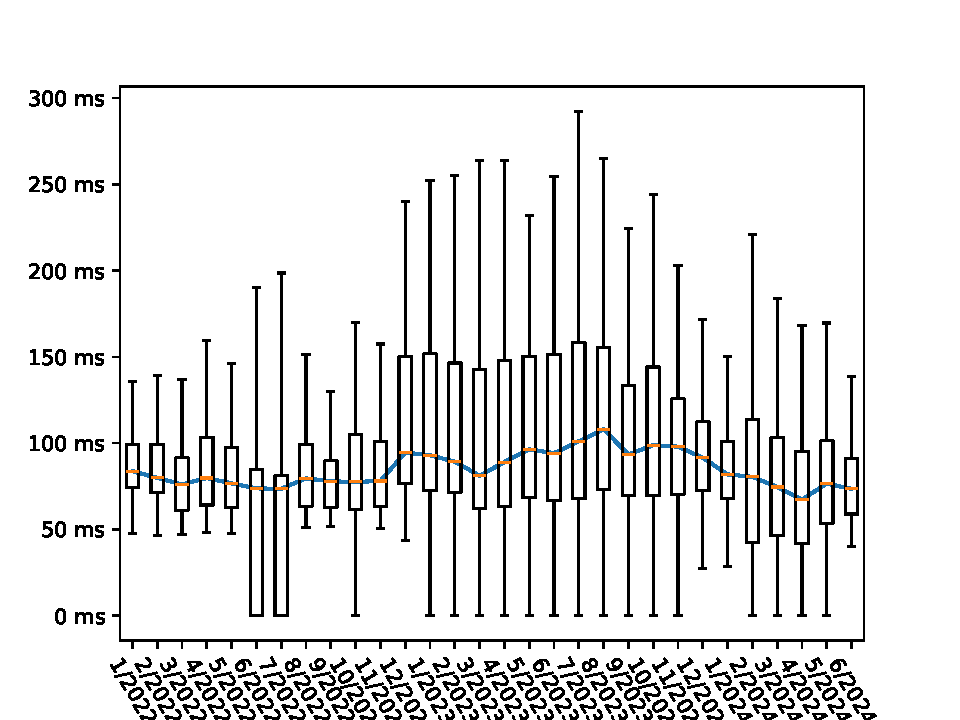
\includegraphics[width=\linewidth]{chapters/4-results/latency/img/latency_2022_to_2024_Germany.pdf}
		\caption{Germany}
	\end{subfigure}
	\begin{subfigure}[b]{0.47\linewidth}
		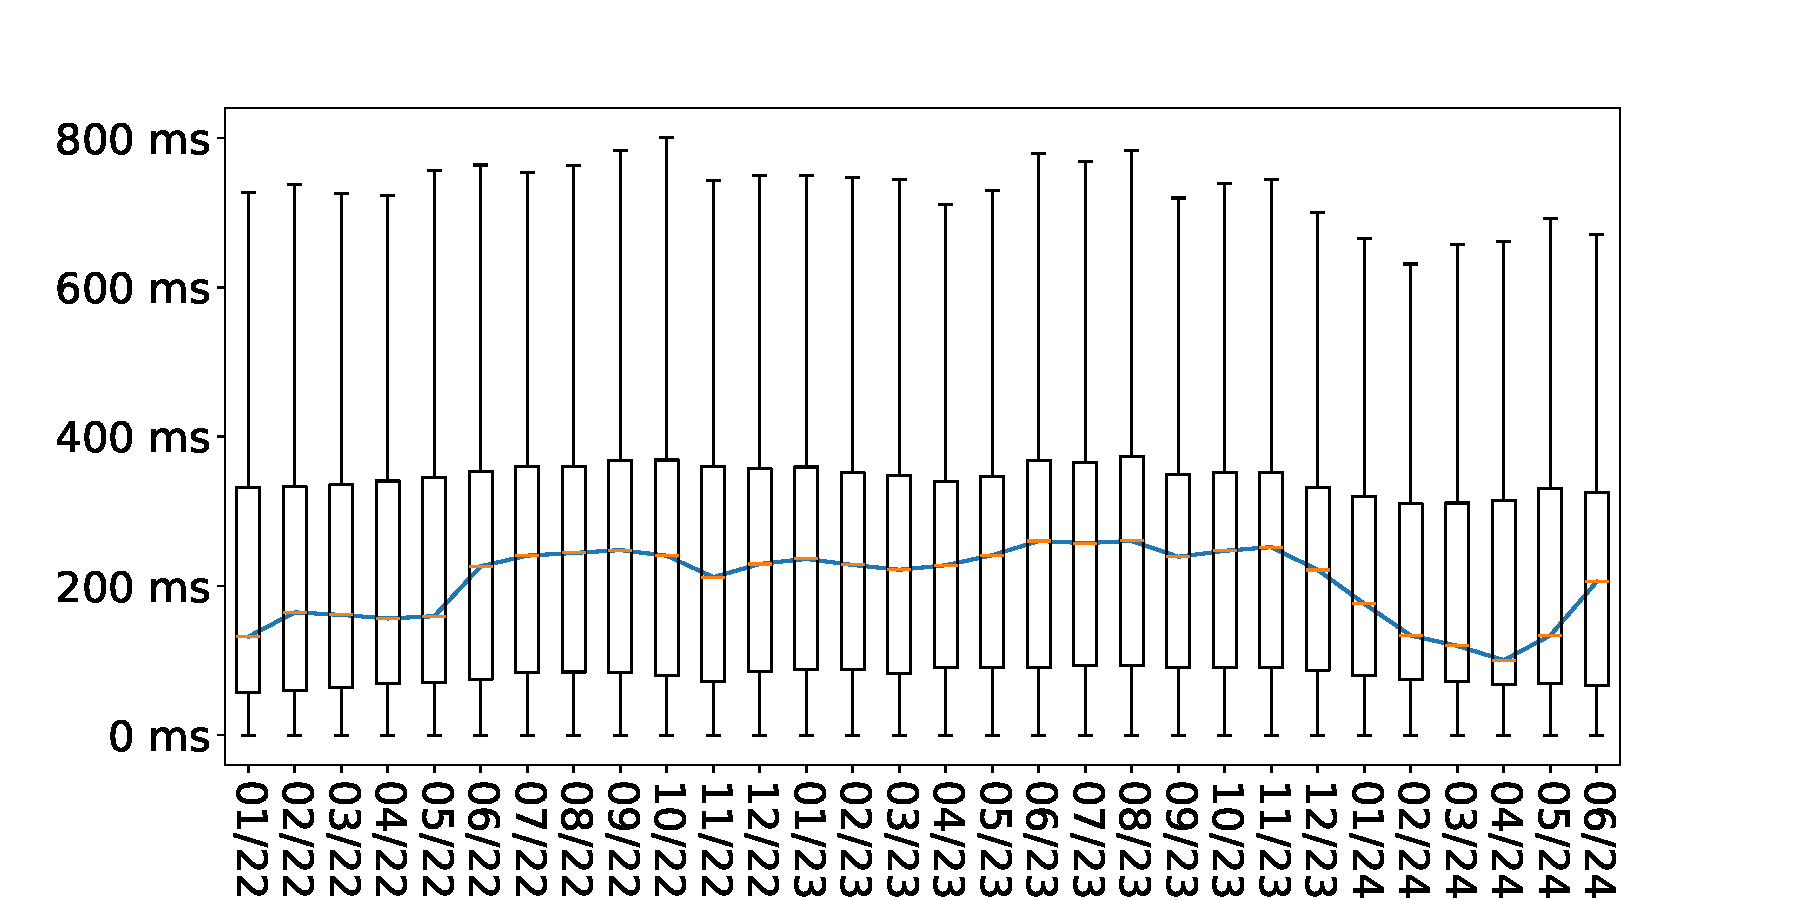
\includegraphics[width=\linewidth]{chapters/4-results/latency/img/latency_2022_to_2024_United States.pdf}
		\caption{USA}
	\end{subfigure}
	\begin{subfigure}[b]{0.47\linewidth}
		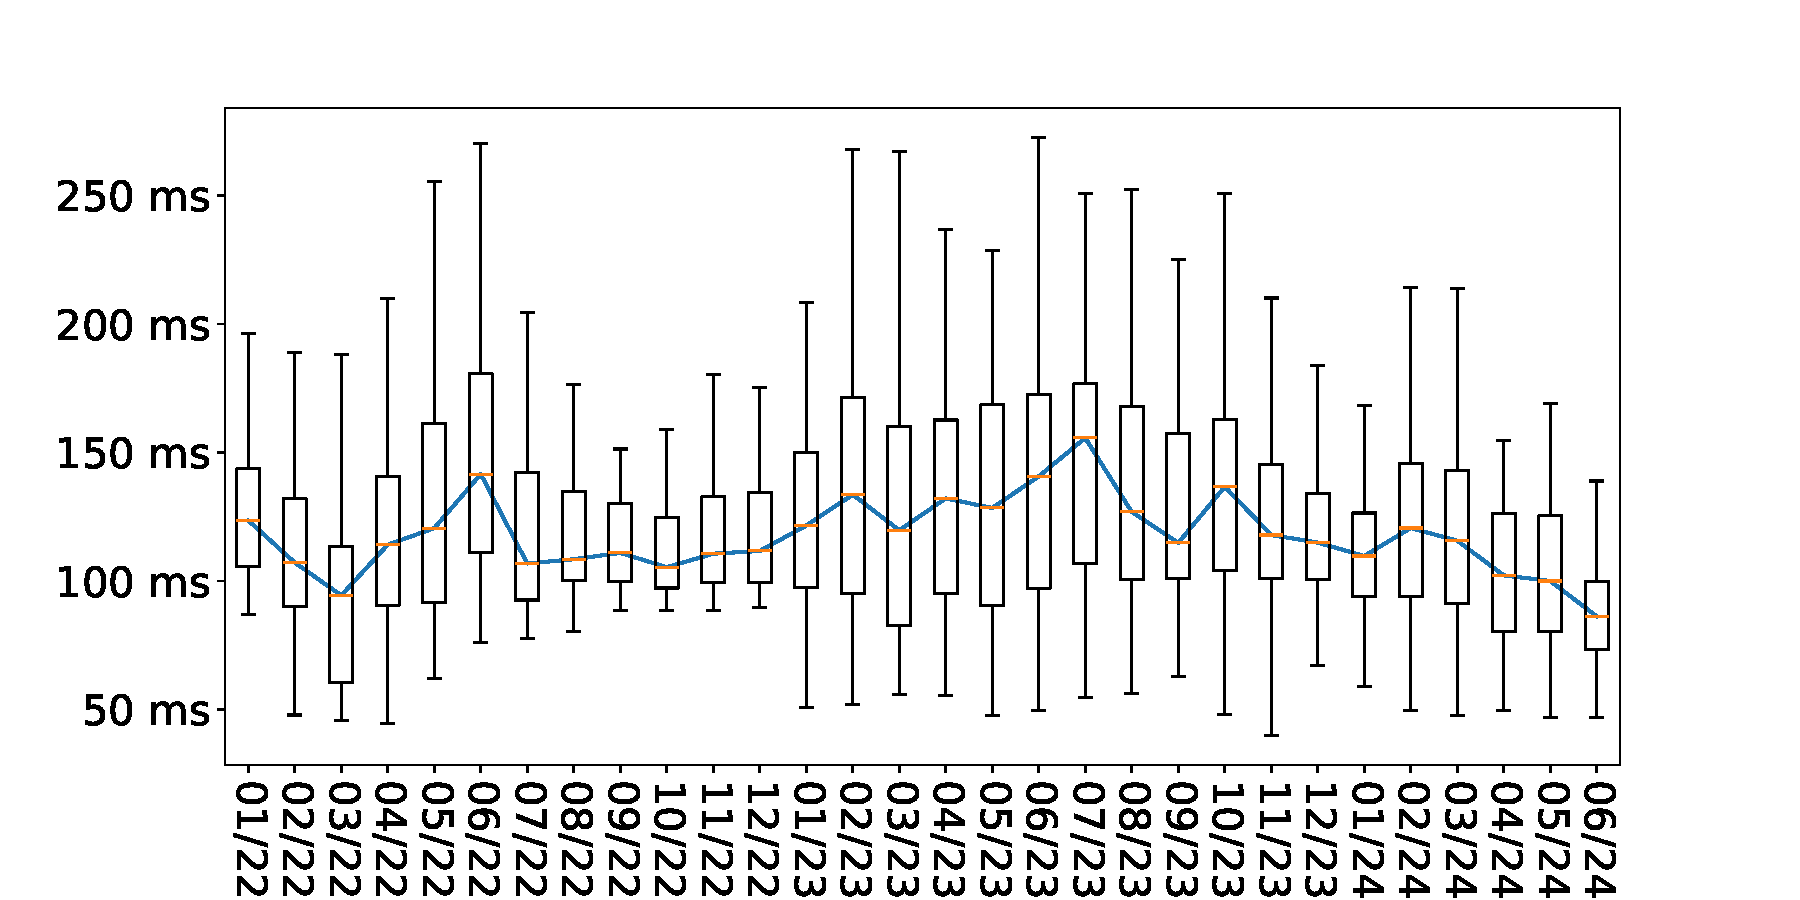
\includegraphics[width=\linewidth]{chapters/4-results/latency/img/latency_2022_to_2024_Poland.pdf}
		\caption{Poland}
	\end{subfigure}
	\begin{subfigure}[b]{0.47\linewidth}
		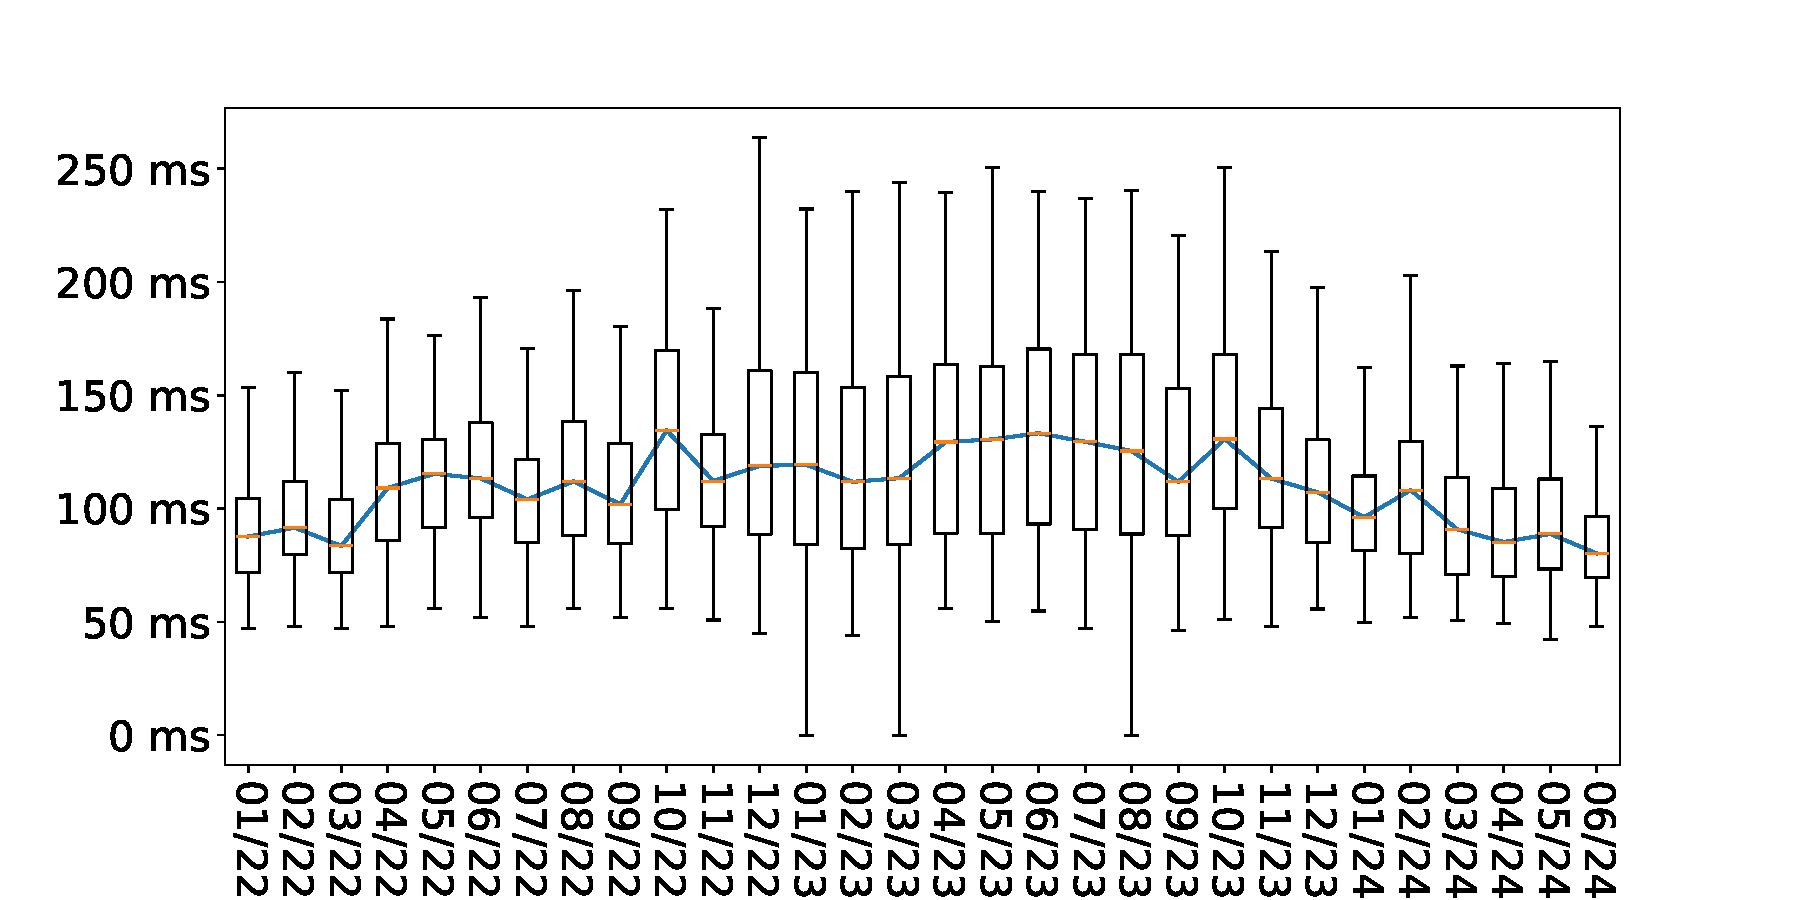
\includegraphics[width=\linewidth]{chapters/4-results/latency/img/latency_2022_to_2024_Austria.pdf}
		\caption{Austria}
	\end{subfigure}
	\caption{Latency History for Germany, the USA, Poland, and Austria in the period 01/2022 to 06/2024}
	\label{fig:latency_wholerange}
\end{figure}

Figure~\ref{fig:latency_wholerange} shows the history of median TLS handshake
latencies from January~2022 until June~2024 for Germany, the United States,
Poland, and Austria\footnote{These countries were chosen due to the
	completeness of data}.

One can see that the median TLS handshake latency is usually at around 100 to 150~ms for most
countries. However, in 2022 the latency was lower compared to 2023. Most of the
countries observed show an upwards trend in the late months of 2022 (most of
the time in December). In the late months of 2023, the latency starts to
decline again. In the last couple of months, we observe an increase in latency
once again. We assume the reason for the rise is the congestion of the Starlink
network. In the recent time, Starlink extended their availability across more
countries allowing more users, especially those in countries with less
networking infrastructure, to access the network. On the contrary, Starlink
also launched more satellites (2022: 3481, 2024: 6000+; see
Chapter~\ref{sec:satellite-constellations}) and added more \ac{PoP} which
likely reduces the congestion.

\begin{figure}
	\centering
	\begin{subfigure}[t]{0.47\linewidth}
		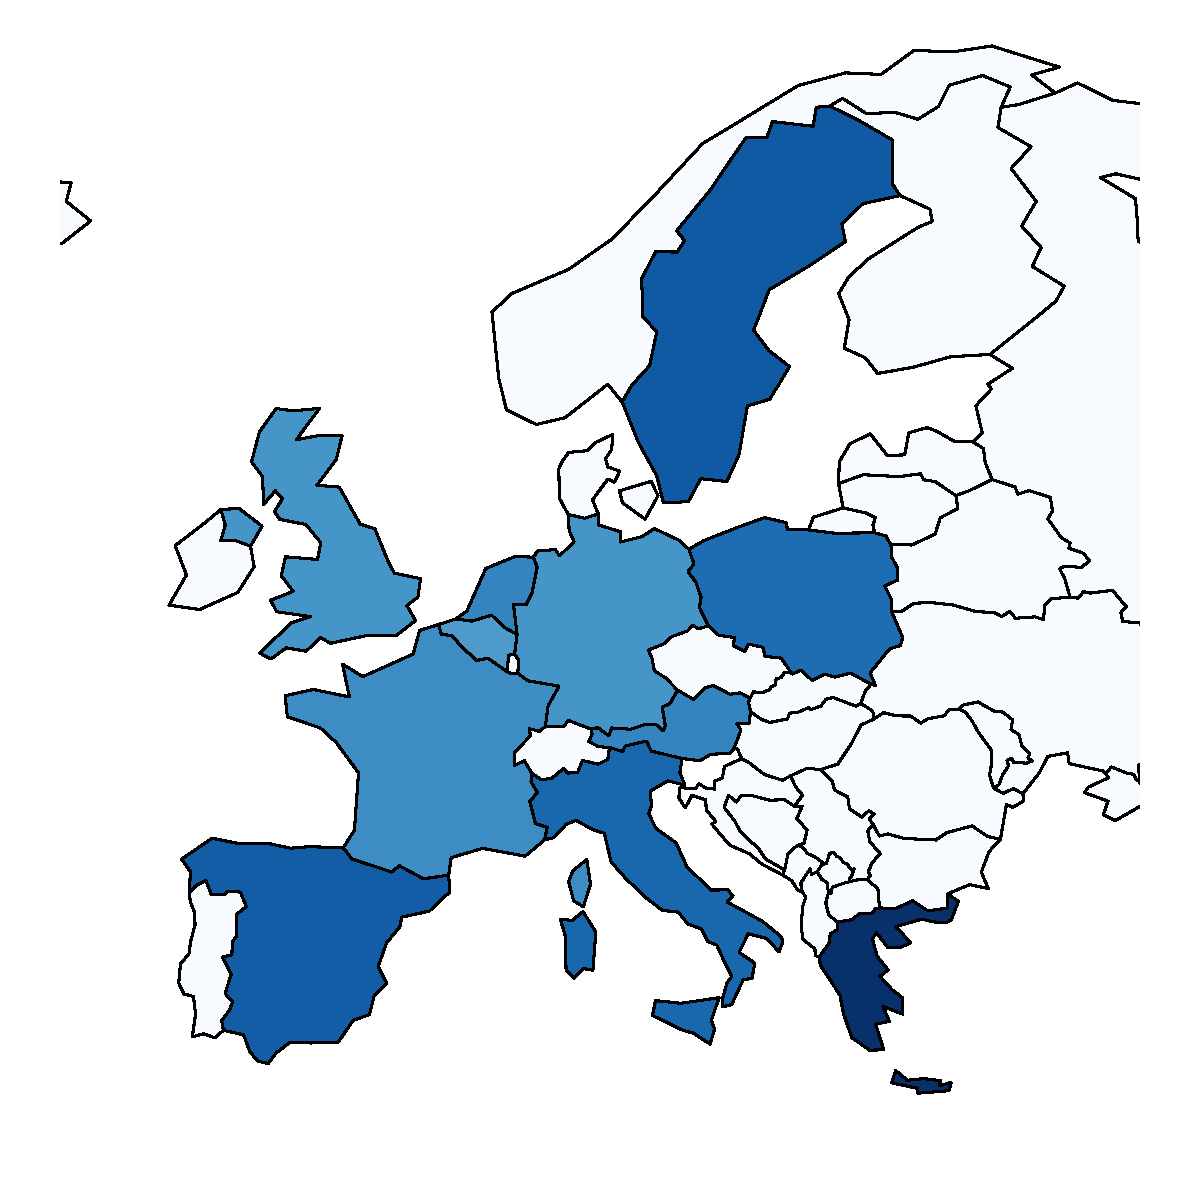
\includegraphics[width=\linewidth]{chapters/4-results/latency/img/heatmap-median-latencies-2024.pdf}
		\caption{Median}
	\end{subfigure}
	\begin{subfigure}[t]{0.47\linewidth}
		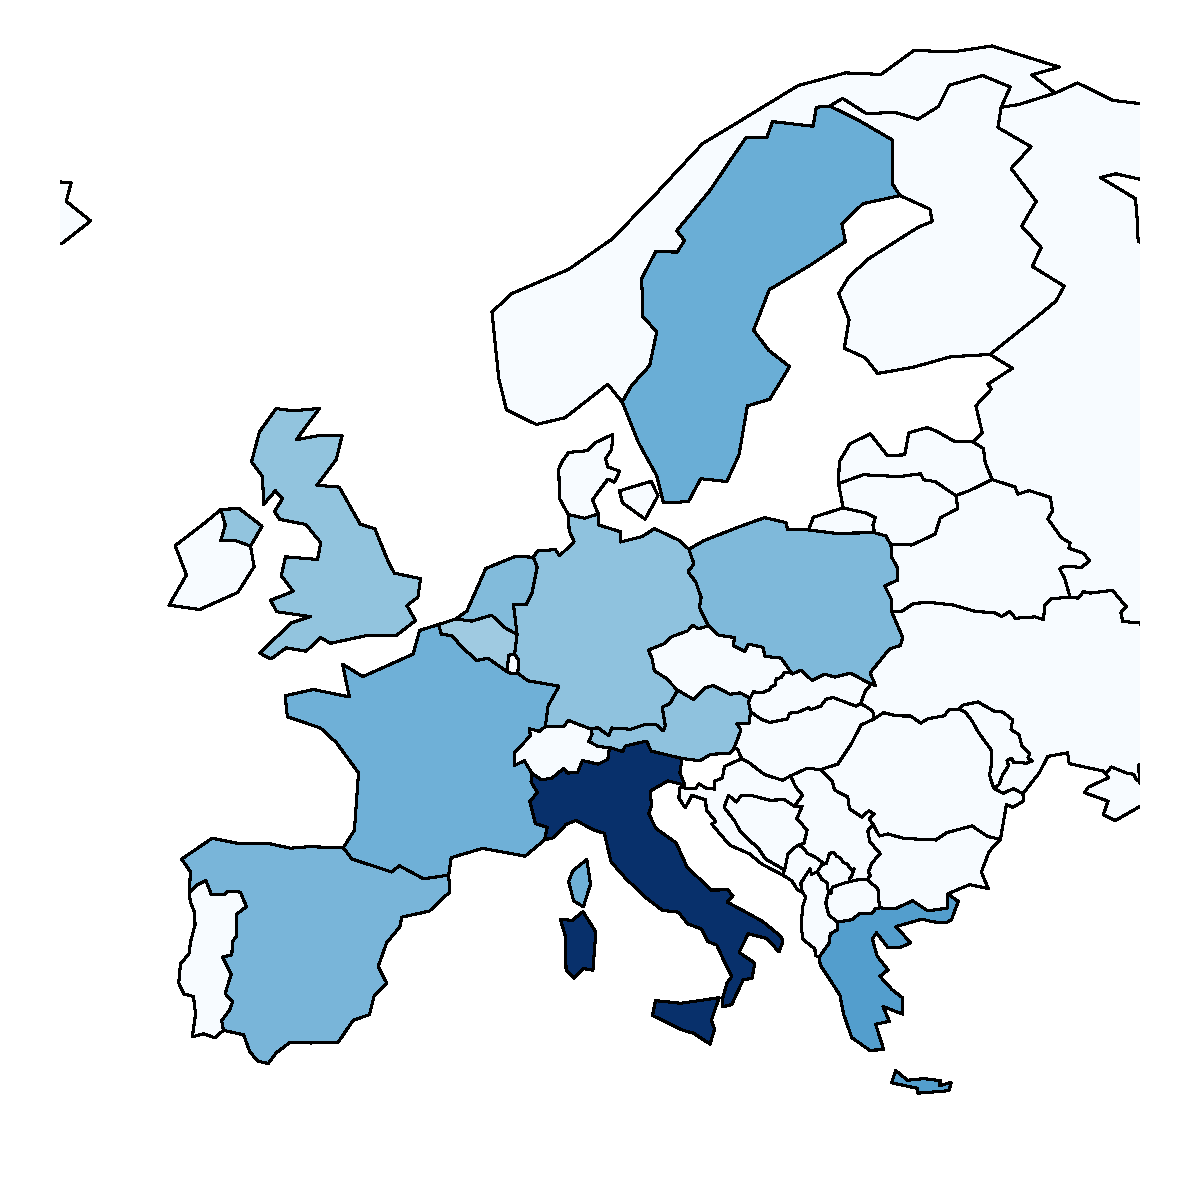
\includegraphics[width=\linewidth]{chapters/4-results/latency/img/heatmap-average-latencies-2024.pdf}
		\caption{Average}
	\end{subfigure}
	\caption{Heatmap of Median and Average Latencies in 2024 in Europe.}
	\label{fig:heatmap-latencies-europe}
\end{figure}

Figure~\ref{fig:heatmap-latencies-europe} shows the median and average TLS
handshake latencies in European countries. It shows that the north west of
Europe experiences the best latencies, likely due to the presence of various
\ac{GS}s. The southern and eastern european countries experience worse
latencies. Especially Greece has a high median latency. A cause could be the
absence of \ac{GS}s in the east-european region. Italy on the other hand side
experiences a high average latency, even with \ac{GS}s being present in the
country.

Looking at the CDFs of the USA and Canada results in a similar observation.
Figure~\ref{fig:latency-cdfs-1} illustrates the CDF plots for 2022 -- 2024
for the USA and Canada. We observe similar results for other countries, but
only chose Canada as it holds sufficient data for a conclusion.

We observe and similar performance of 2022 and 2024, but a drop in TLS
handshake latency in 2023, similar to the conclusion we drew before.

Additionally, we conclude that approximately half of the measurement results
are below 100 ms, while the other half moves above 100 ms. This opposes
research suggesting Starlink performance is mostly in the sub-100 ms area
\cite{DBLP:conf/www/MohanFCBRMO24, DBLP:conf/icnp/LaiLL20,
	DBLP:journals/pacmnet/RamanVCSZ23, DBLP:conf/imc/MichelTGB22}.

The CDF is continuous, up to a specific point, where it flattens, followed by a
stronger increase once again. This is similarly observed for curves of other
countries (e.g., for France and Germany in Figure~\ref{fig:latency-cdfs-2}).
This observation suggests that there is a region of latencies that Starlink
does not serve equally. The specific location of the flattening behavior varies
between countries, but is usually located between 150 and 250 ms.

\begin{figure}
	\centering
	\begin{subfigure}[b]{0.8\linewidth}
		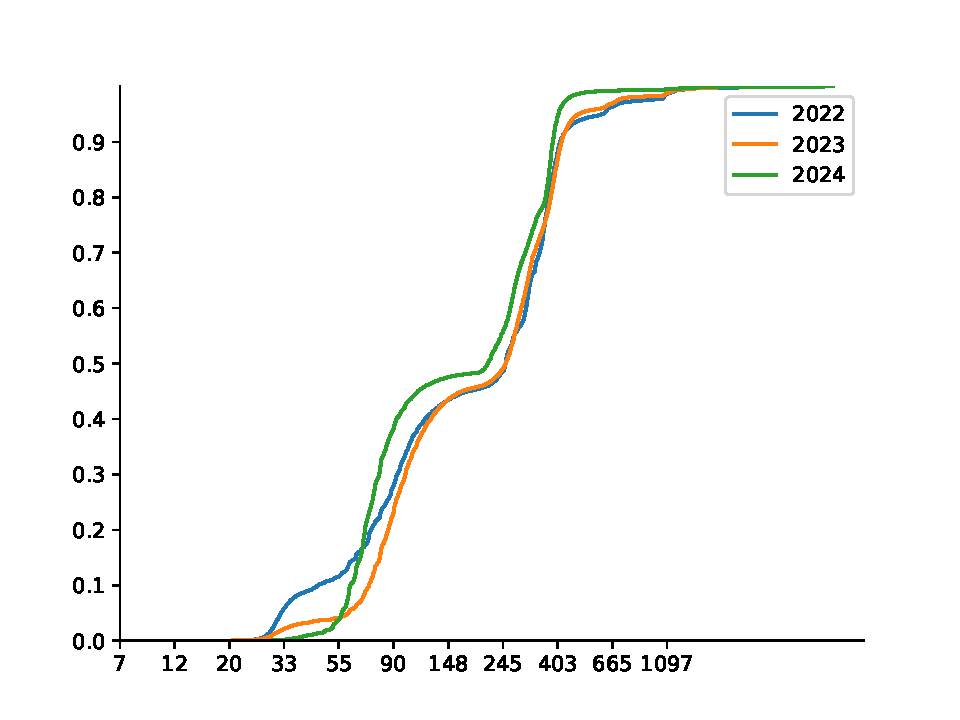
\includegraphics[width=\linewidth]{chapters/4-results/latency/img/cdf_latencies_of_starlink_probes_in_united_states.pdf}
		\caption{USA}
	\end{subfigure}
	\begin{subfigure}[b]{0.8\linewidth}
		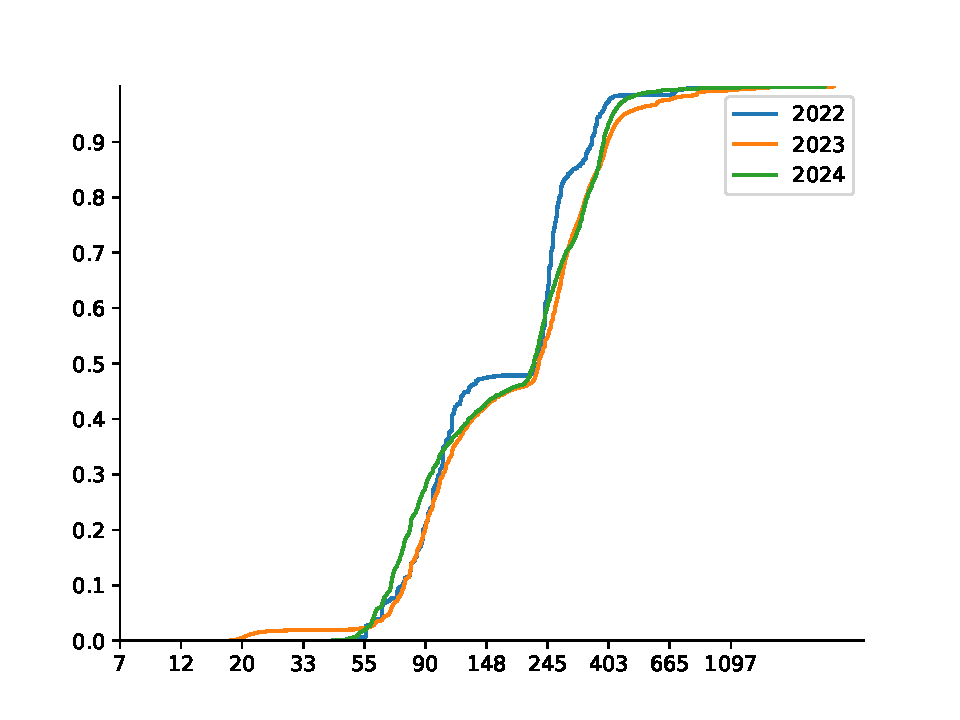
\includegraphics[width=\linewidth]{chapters/4-results/latency/img/cdf_latencies_of_starlink_probes_in_canada.pdf}
		\caption{Canada}
	\end{subfigure}
	\caption{CDF of Latencies in the USA and Canada}
	\label{fig:latency-cdfs-1}
\end{figure}

\begin{figure}
	\centering
	\begin{subfigure}[b]{0.8\linewidth}
		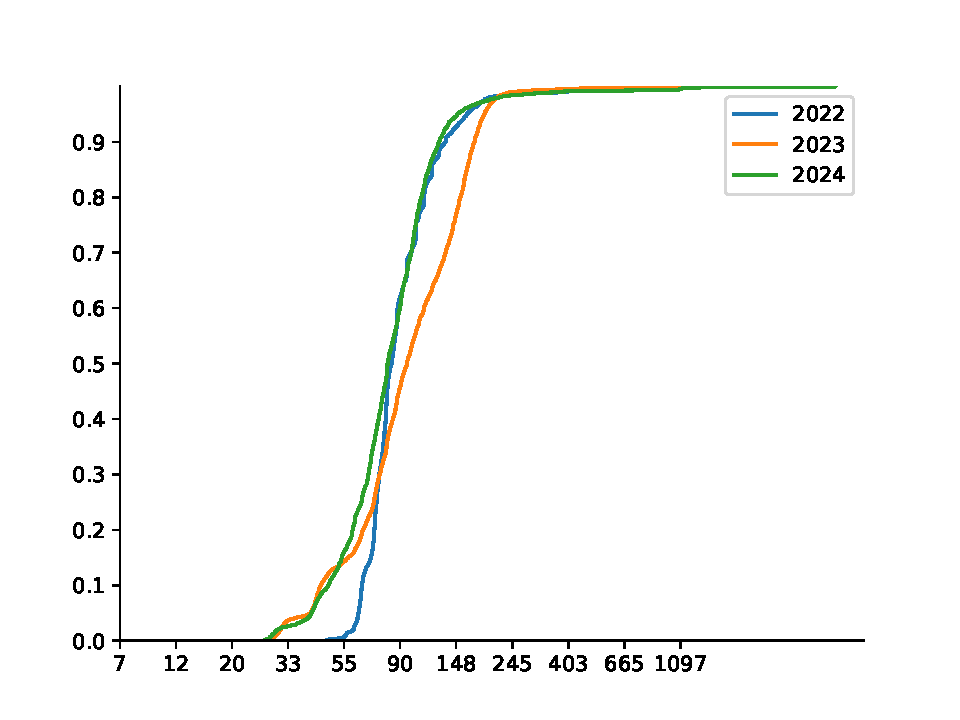
\includegraphics[width=\linewidth]{chapters/4-results/latency/img/cdf_latencies_of_starlink_probes_in_germany.pdf}
		\caption{Germany}
	\end{subfigure}
	\begin{subfigure}[b]{0.8\linewidth}
		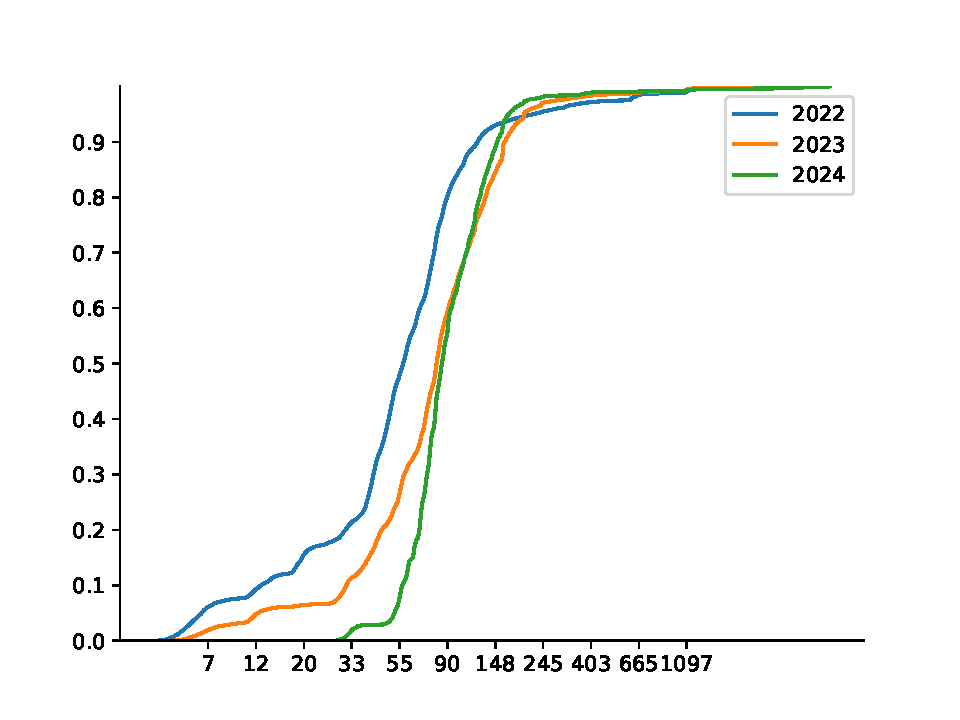
\includegraphics[width=\linewidth]{chapters/4-results/latency/img/cdf_latencies_of_starlink_probes_in_france.pdf}
		\caption{France}
	\end{subfigure}
	\caption{CDF of Latencies in Germany and France}
	\label{fig:latency-cdfs-2}
\end{figure}

\begin{figure}
	\centering
	\begin{subfigure}[b]{0.8\linewidth}
		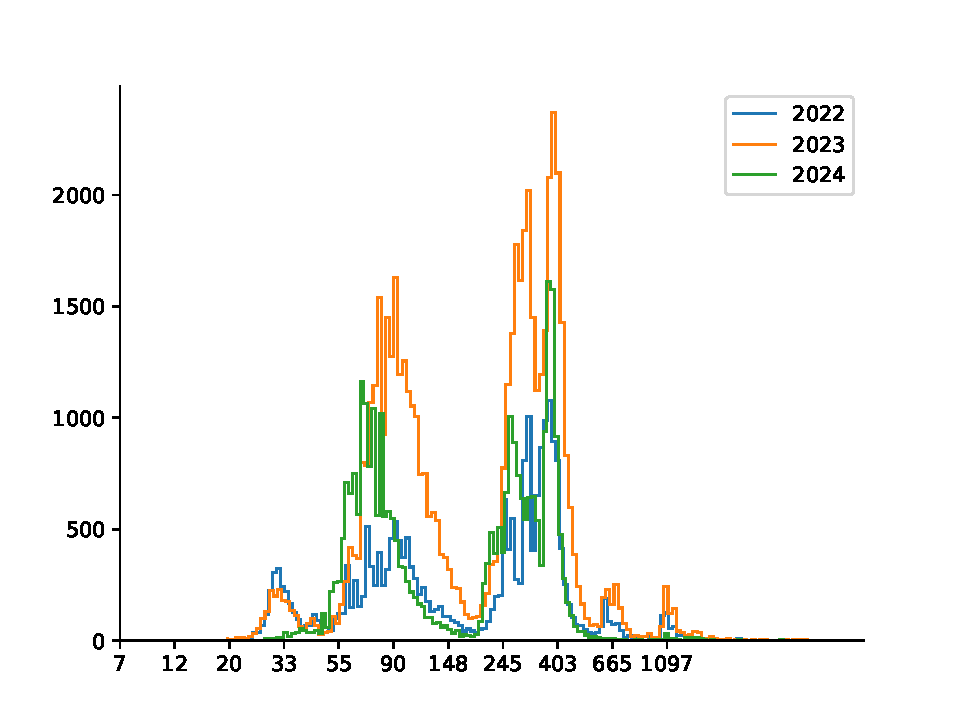
\includegraphics[width=\linewidth]{chapters/4-results/latency/img/histogram_of_latencies_of_starlink_probes_in_united_states.pdf}
		\caption{USA}
	\end{subfigure}
	\begin{subfigure}[b]{0.8\linewidth}
		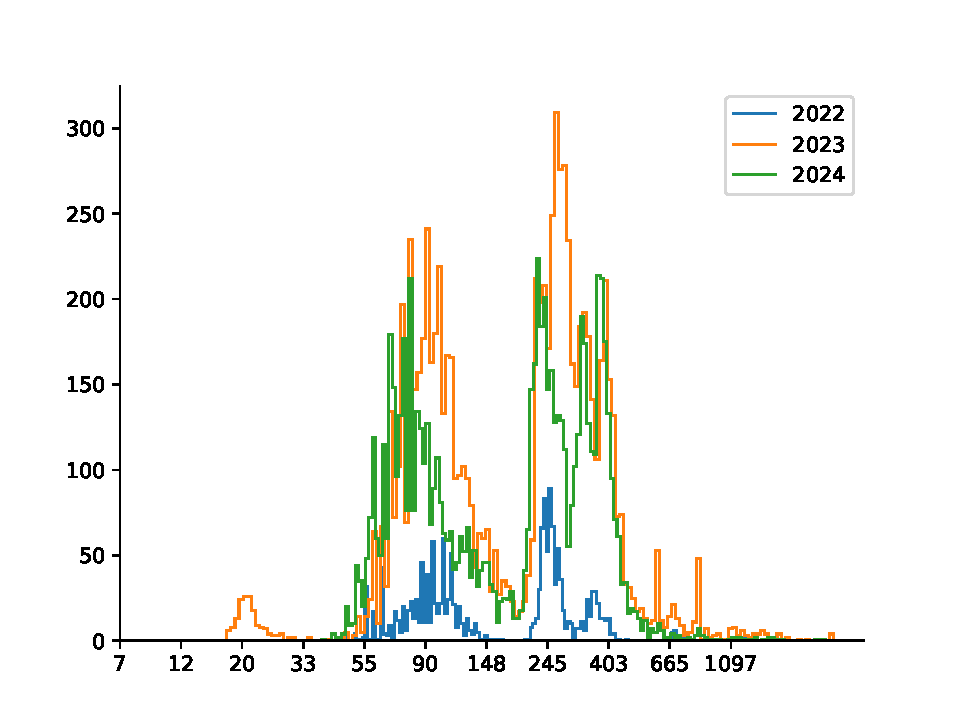
\includegraphics[width=\linewidth]{chapters/4-results/latency/img/histogram_of_latencies_of_starlink_probes_in_canada.pdf}
		\caption{Canada}
	\end{subfigure}
	\caption{EquiWidth Histogram of Latencies in the USA and Canada}
	\label{fig:latency-histogram-1}
\end{figure}

\begin{figure}
	\centering
	\begin{subfigure}[b]{0.8\linewidth}
		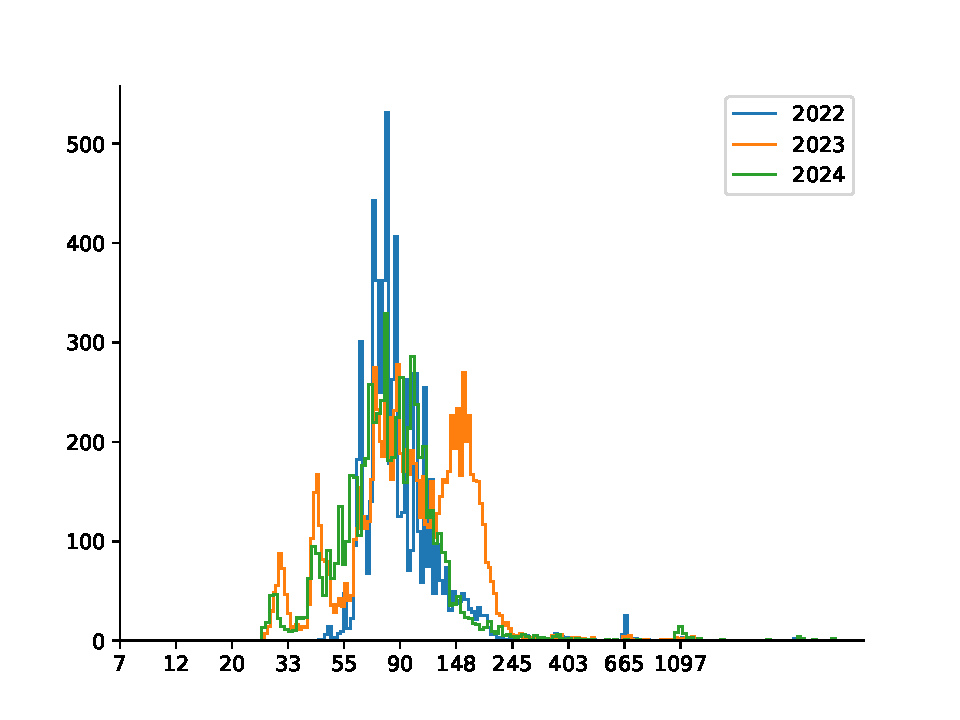
\includegraphics[width=\linewidth]{chapters/4-results/latency/img/histogram_of_latencies_of_starlink_probes_in_germany.pdf}
		\caption{Germany}
	\end{subfigure}
	\begin{subfigure}[b]{0.8\linewidth}
		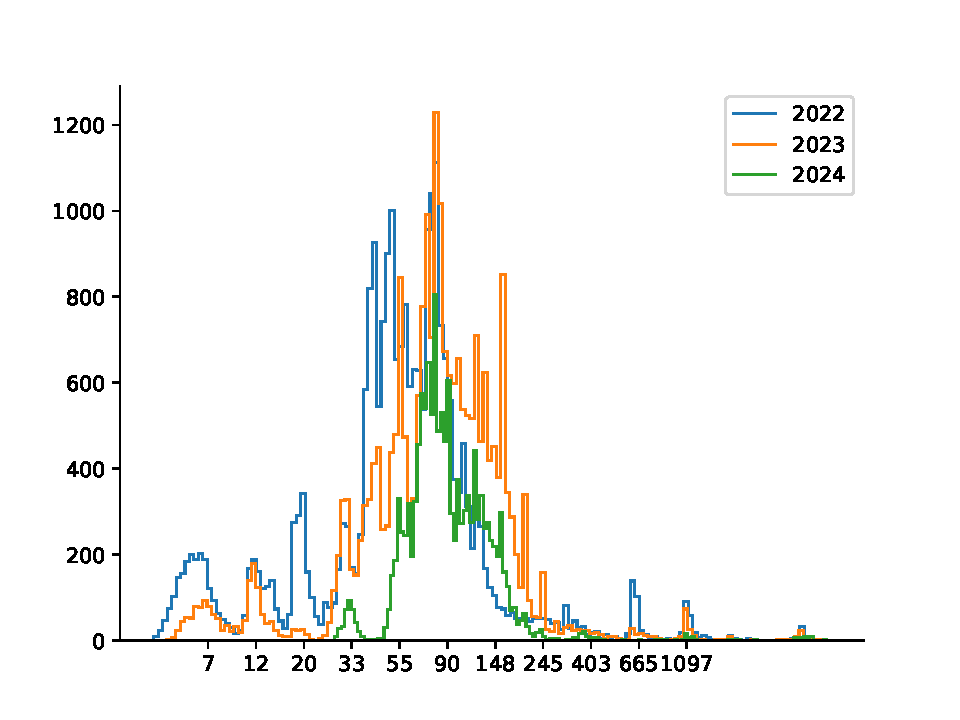
\includegraphics[width=\linewidth]{chapters/4-results/latency/img/histogram_of_latencies_of_starlink_probes_in_france.pdf}
		\caption{France}
	\end{subfigure}
	\caption{EquiWidth Histogram of Latencies in Germany and France}
	\label{fig:latency-histogram-2}
\end{figure}

Analyzing the flattening behavior in more detail, we used an EquiWidth
histogram\footnote{A histogram that puts all values in a pre-defined number of
	bins, where all bins cover an equally wide data-range.} to plot the
most frequent latencies. Figure~\ref{fig:latency-histogram-1} and
\ref{fig:latency-histogram-2} show the histograms for the USA, Canada, France,
and Germany. It becomes apparent that there is actually a major gap between
within the latencies. This gap appears for most countries. In 2024, it became
even more apparent (e.g., looking at Germany, the gap was not visible in 2022,
but appeared in 2024). For further countries, the appendix holds further plots
(see Figures~\ref{fig:latency-cdf-3} -- \ref{fig:latency-cdf-7} and
\ref{fig:latency-histogram-3} -- \ref{fig:latency-histogram-7}).

Currently, it is unclear why the gap appears, but we assume that either
the measurements were consistent enough for such a pattern to occur or the gap
is a special trait of the Starlink system. The latter would infer that Starlink
serves specific latencies better than others.

